\section{Group -- Air Path}\label{group-air-path}

\subsection{AirLoopHVAC:SupplyPath, AirLoopHVAC:ReturnPath}\label{airloophvacsupplypath-airloophvacreturnpath}

The zone supply and return air paths are used to describe the configuration of the flow path that the supply air takes in moving from the main air handler to the zone terminal units and that the return air takes on leaving the zones and returning to the central return air duct. The air paths consist of a group of components \hyperref[airloophvaczonesplitter]{AirLoopHVAC:ZoneSplitter}s and \hyperref[airloophvacsupplyplenum]{AirLoopHVAC:SupplyPlenum}s for the supply path and \hyperref[airloophvacreturnplenum]{AirLoopHVAC:ReturnPlenum}s and \hyperref[airloophvaczonemixer]{AirLoopHVAC:ZoneMixer}s for the return path. The connectivity of the paths is established by the components node connections. There are no branches defined in the zone air path constructs.

For a typical single duct air system there will be one \hyperref[airloophvacsupplypath]{AirLoopHVAC:SupplyPath} and one \hyperref[airloophvacreturnpath]{AirLoopHVAC:ReturnPath}. A typical dual duct system would have 2 \hyperref[airloophvacsupplypath]{AirLoopHVAC:SupplyPath}s one for the hot air and one for the cold air and 1 \hyperref[airloophvacreturnpath]{AirLoopHVAC:ReturnPath}.

The \hyperref[airloophvacsupplyplenum]{AirLoopHVAC:SupplyPlenum} component provides the capability to have supply air distributed to the conditioned zones through one or more plenum zones such as would occur in an underfloor air distribution system (UFAD). The \hyperref[airloophvacreturnplenum]{AirLoopHVAC:ReturnPlenum} component allows the program to model return air plenums. Of course plenums are always optional. The simplest \hyperref[airloophvacsupplypath]{AirLoopHVAC:SupplyPath} would consist of only an \hyperref[airloophvaczonesplitter]{AirLoopHVAC:ZoneSplitter}; similarly the simplest return air path consists of a single \hyperref[airloophvaczonemixer]{AirLoopHVAC:ZoneMixer}. A UFAD system supply air path might consist of a single \hyperref[airloophvaczonesplitter]{AirLoopHVAC:ZoneSplitter} connecting to multiple \hyperref[airloophvacsupplyplenum]{AirLoopHVAC:SupplyPlenum}s which in turn could each supply one or more conditioned zones. A system with return plenums would have an \hyperref[airloophvacreturnpath]{AirLoopHVAC:ReturnPath} in which the conditioned zones connect to the return plenum inlets and the outlets of the return plenum connect to a single \hyperref[airloophvaczonemixer]{AirLoopHVAC:ZoneMixer}.

Both the zone supply and return plenums are solved in the heat balance as thermal zones which couple through heat conduction with adjacent zones. Since they are solved as thermal zones the solution scheme involves the zone predictor-corrector technique which will lag the temperature at the system timestep in every zone. See Summary of Predictor-Corrector Procedure in the EnergyPlus Engineering Reference.

Below are the descriptions of the zone supply and return path statements. Note that each statement type has an identifying name, a single inlet/outlet node name, and a list of component type/name pairs. For a single zone being served by an air loop, the inlet to its air distribution unit and the zone return air outlet can be the zone equipment inlet and outlet nodes directly, thus eliminating the need to specify an \hyperref[airloophvacsupplypath]{AirLoopHVAC:SupplyPath} and an \hyperref[airloophvacreturnpath]{AirLoopHVAC:ReturnPath}.

\subsection{AirLoopHVAC:SupplyPath}\label{airloophvacsupplypath}

The AirLoopHVAC:SupplyPath lists one or more \hyperref[airloophvaczonesplitter]{AirLoopHVAC:ZoneSplitter} and \hyperref[airloophvacsupplyplenum]{AirLoopHVAC:SupplyPlenum} components comprising the path. The components are listed in flow order: upstream to downstream and may be in series, parallel, or both. Connectivity is established by means of the individual component inlet and outlet nodes.

\subsubsection{Inputs}\label{inputs-003}

\paragraph{Field: Name}\label{field-name-003}

Unique name to identify the supply air path..

\paragraph{Field: Supply Air Path Inlet Node Name}\label{field-supply-air-path-inlet-node-name}

The name of an inlet node for the zone equipment half of the air loop. This should be one of the nodes named in the \hyperref[airloophvac]{AirLoopHVAC} field: Demand Side Inlet Node Names.

\paragraph{Field Set Component Type and Name}\label{field-set-component-type-and-name}

The remaining fields are sets of two repeated times: a component type and a name. These pairs of fields define the components on the supply air path.

\paragraph{Field: Component \textless{}\#\textgreater{} Object Type}\label{field-component-object-type}

Start of the component list for the AirLoopHVAC:SupplyPath. This field should contain either \emph{\hyperref[airloophvacsupplyplenum]{AirLoopHVAC:SupplyPlenum}} or \emph{\hyperref[airloophvaczonesplitter]{AirLoopHVAC:ZoneSplitter}}.

\paragraph{Field: Component \textless{}\#\textgreater{} Name}\label{field-component-name}

Unique name of the \hyperref[airloophvacsupplyplenum]{AirLoopHVAC:SupplyPlenum} or \hyperref[airloophvaczonesplitter]{AirLoopHVAC:ZoneSplitter} component.

\subsection{AirLoopHVAC:ReturnPath}\label{airloophvacreturnpath}

The AirLoopHVAC:ReturnPath lists one or more \hyperref[airloophvaczonemixer]{AirLoopHVAC:ZoneMixer} and \hyperref[airloophvacreturnplenum]{AirLoopHVAC:ReturnPlenum} components comprising the path. The components are listed in flow order: upstream to downstream and may be in series, parallel, or both. Connectivity is established by means of the individual component inlet and outlet nodes. At this time there can only be 1 \hyperref[airloophvaczonemixer]{AirLoopHVAC:ZoneMixer} in an AirLoopHVAC:ReturnPath.

\subsubsection{Inputs}\label{inputs-1-003}

\paragraph{Field: Name}\label{field-name-1-002}

Unique name to identify the return air path.

\paragraph{Field: Return Air Path Outlet Node Name}\label{field-return-air-path-outlet-node-name}

The name of the node that is the outlet to the air loop from the AirLoopHVAC:ReturnPath. This should be the same node named in the \hyperref[airloophvac]{AirLoopHVAC} field: Demand Side Outlet Node Name.

\paragraph{Field Set Component Type and Name}\label{field-set-component-type-and-name-1}

The remaining fields are sets of two repeated times: a component type and a name. These pairs of fields define the components on the return air path.

\paragraph{Field: Component \textless{}\#\textgreater{} Object Type}\label{field-component-object-type-1}

Start of the component list for the AirLoopHVAC:ReturnPath. This field should contain either \emph{\hyperref[airloophvacreturnplenum]{AirLoopHVAC:ReturnPlenum}} or \emph{\hyperref[airloophvaczonemixer]{AirLoopHVAC:ZoneMixer}}.

\paragraph{Field: Component \textless{}\#\textgreater{} Name}\label{field-component-name-1}

Unique name of the \hyperref[airloophvacreturnplenum]{AirLoopHVAC:ReturnPlenum} or \hyperref[airloophvaczonemixer]{AirLoopHVAC:ZoneMixer}.

Example inputs are shown below

\begin{lstlisting}

AirLoopHVAC:SupplyPath,
  SupplyAirPath 1,              !- Name
  Zone Equip In Node,           !- Supply Air Path Inlet Node Name
  AirLoopHVAC:SupplyPlenum,     !- Component 1 Object Type
  Supply-Plenum-1,              !- Component 1 Name
  AirLoopHVAC:ZoneSplitter,     !- Component 2 Object Type
  Zone Supply Air Splitter 1;   !- Component 2 Name


  AirLoopHVAC:ReturnPath,
  ReturnAirPath1,               !- Name
  PLENUM-1 Out Node,            !- Return Air Path Outlet Node Name
  Zone Return Plenum,           !- Component 1 Object Type
  Return-Plenum-1;              !- Component 1 Name
\end{lstlisting}

\subsection{AirLoopHVAC:ReturnPlenum}\label{airloophvacreturnplenum}

The simple building shown in the figure below consists of a controlled zone and a return plenum zone that is used for the return air. This simple configuration contains a ground floor controlled zone with a window and a return plenum zone which handles the roof load. The return air plenum is a special type of component since there is both a heat balance connection and building description and a system airflow connection that transfers the airflow directly from the controlled zone to the return plenum zone in the system air simulation. The input described in this section is mainly just for the system airflow connections in the HVAC algorithms. In addition the return plenum zone must be fully input as a zone object for the heat balance calculation. The zone description needs to contain the wall descriptions - the interzone ceiling and floor, and for this simple case the roof. All the other attributes of a zone that can be specified in the building description can be used with a return plenum zone if necessary: scheduled loads, windows, etc.

\begin{figure}[hbtp] % fig 130
\centering
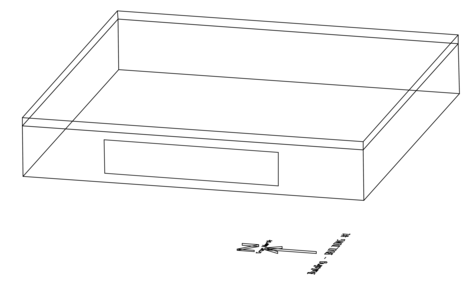
\includegraphics[width=0.9\textwidth, height=0.9\textheight, keepaspectratio=true]{media/image337.png}
\caption{Illustration of Zone Return Plenum \protect \label{fig:illustration-of-zone-return-plenum}}
\end{figure}

After all the building zone attributes are specified, the AirLoopHVAC:ReturnPlenum object is specified and included as one of the named components in an \hyperref[airloophvacreturnpath]{AirLoopHVAC:ReturnPath}.

\subsubsection{Inputs}\label{inputs-2-003}

\paragraph{Field: Name}\label{field-name-2-002}

A unique identifying name identifying the AirLoopHVAC:ReturnPlenum system component.

\paragraph{Field: Zone Name}\label{field-zone-name-000}

The zone name specified in the heat balance portion of the input. This piece of input connects the zone return plenum system component to the heat balance data structure.

\paragraph{Field: Zone Node Name}\label{field-zone-node-name}

The name of the zone node. The zone node name connects the heat balance data structure to the system airflow data structure through this node. This node name must be unique otherwise a warning is reported. Do not use the Zone Air Node Name specified in any \hyperref[zonehvacequipmentconnections]{ZoneHVAC:EquipmentConnections} object, and since this zone is a plenum a \hyperref[zonehvacequipmentconnections]{ZoneHVAC:EquipmentConnections} object is not required for the zone named in the previous field.

\paragraph{Field: Outlet Node Name}\label{field-outlet-node-name-000}

The name of the return plenum outlet node. For the zone return plenum there is only one outlet node that can be specified.

\paragraph{Field: Induced Air Outlet Node or NodeList Name}\label{field-induced-air-outlet-node-or-nodelist-name}

The name of an induced air outlet node or the name of a \hyperref[nodelist]{NodeList} of such nodes. These nodes are to be used as the secondary inlet air nodes of powered induction terminal units (See \textbf{\hyperref[airterminalsingleductseriespiureheat]{AirTerminal:SingleDuct:SeriesPIU:Reheat}} and \textbf{\hyperref[airterminalsingleductparallelpiureheat]{AirTerminal:SingleDuct:ParallelPIU:Reheat}}).

\paragraph{Field: Inlet \textless{}\#\textgreater{} Node Name}\label{field-inlet-node-name}

The name of a plenum inlet node. There is no limit to the number of inlet nodes, and there may be no duplicate inlet node names.  This object is extensible, so additional fields of this type can be added to the end of this object.  (Note that some EnergyPlus editing tools may allow only 500 inlet node names.)

An IDF example of a zone return plenum component specification:

\begin{lstlisting}

AirLoopHVAC:ReturnPlenum,
  Return-Plenum-1,            !- Name
  PLENUM-1,                   !- Zone Name
  PLENUM-1 Node,              !- Zone Node Name
  PLENUM-1 Out Node,          !- Outlet Node Name
  PLENUM-1 Induced Air Nodes, !- Induced Air Outlet Node or NodeList Name
  SPACE1-1 Out Node,          !- Inlet 1 Node Name
  SPACE2-1 Out Node,          !- Inlet 2 Node Name
  SPACE3-1 Out Node,          !- Inlet 3 Node Name
  SPACE4-1 Out Node,          !- Inlet 4 Node Name
  SPACE5-1 Out Node;          !- Inlet 5 Node Name


  NodeList,
  PLENUM-1 Induced Air Nodes, !- Name
  SPACE1-1 ATU Sec Node,      !- Node 1 Name
  SPACE2-1 ATU Sec Node,      !- Node 2 Name
  SPACE3-1 ATU Sec Node,      !- Node 3 Name
  SPACE4-1 ATU Sec Node;      !- Node 4 Name
\end{lstlisting}

Below is an example of the \hyperref[airloophvacreturnpath]{AirLoopHVAC:ReturnPath} for the simple case shown above.

\begin{lstlisting}

AirLoopHVAC:ReturnPath,
  ReturnAirPath1,              !- Name
  PLENUM-1 Out Node,           !- Return Air Path Outlet Node Name
  AirLoopHVAC:ReturnPlenum,    !- Component 1 Object Type
  Return-Plenum-1;             !- Component 1 Name
\end{lstlisting}

\subsection{AirLoopHVAC:SupplyPlenum}\label{airloophvacsupplyplenum}

The building shown in the figure below consists of three controlled zones served by an AirLoopHVAC:SupplyPlenum beneath the floor.

\begin{figure}[hbtp] % fig 131
\centering
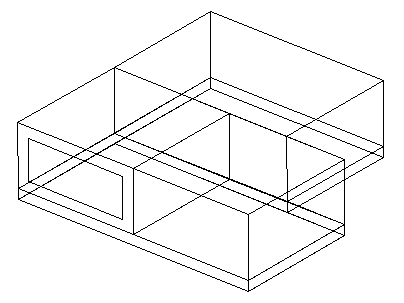
\includegraphics[width=0.9\textwidth, height=0.9\textheight, keepaspectratio=true]{media/image338.png}
\caption{Illustration of AirLoopHVAC:SupplyPlenum \protect \label{fig:illustration-of-airloophvac-supplyplenum}}
\end{figure}

The AirLoopHVAC:SupplyPlenum has a heat balance connection and building description, and a system airflow connection which transfers the airflow from the supply plenum zone to the controlled zones in the system simulation. The input described in this section is mainly just for the system airflow connections in the HVAC algorithms. In addition the supply plenum zone must be fully input in the building zone description. The supply plenum zone description needs to contain the wall descriptions, the interzone ceiling and floor, and the ground connection. All the other attributes of a zone that can be specified in the building description can be utilized with a supply plenum zone if necessary, i.e.~scheduled loads, windows, etc.

After all the building zone attributes are specified, the AirLoopHVAC:SupplyPlenum object is specified and included as one of the named components in an \hyperref[airloophvacsupplypath]{AirLoopHVAC:SupplyPath}.

\subsubsection{Inputs}\label{inputs-3-002}

\paragraph{Field: Name}\label{field-name-3-002}

A unique identifying name identifying the AirLoopHVAC:SupplyPlenum system component.

\paragraph{Field: Zone Name}\label{field-zone-name-1}

The zone name specified in the heat balance portion of the input. This piece of input connects the AirLoopHVAC:SupplyPlenum system component to the heat balance data structure.

\paragraph{Field: Zone Node Name}\label{field-zone-node-name-1}

The name of the zone node. The zone node name connects the heat balance data structure to the system airflow data structure through this node. This node name is defined by the user in the field Zone Air Node Name in the \hyperref[zonehvacequipmentconnections]{ZoneHVAC:EquipmentConnections} object for the zone named in the previous field.

\paragraph{Field: Inlet Node Name}\label{field-inlet-node-name-1}

The name of the inlet node to the supply plenum. The AirLoopHVAC:SupplyPlenum component can send air to many outlets, but there is only one inlet.

\paragraph{Field: Outlet \textless{}\#\textgreater{} Node Name}\label{field-outlet-node-name-1-000}

The name of a plenum outlet node. There is no limit to the number of outlet nodes, and there may be no duplicate outlet node names.  This object is extensible, so additional fields of this type can be added to the end of this object. (Note that some EnergyPlus editing tools may allow only 500 outlet node names.)

An IDF example of an AirLoopHVAC:SupplyPlenum component specification:

\begin{lstlisting}

AirLoopHVAC:SupplyPlenum,
  Supply Plenum 1,                         ! Name
  SUPPLY PLENUM ZONE,                   ! Zone Name
  Supply Plenum 1 Zone Node,     ! Zone Node Name
  Zone Equipment Inlet Node,     ! Inlet Node Name
  Supply Plenum 1 Outlet Node; ! Outlet 1 Node Name
\end{lstlisting}

Below is an example of the \hyperref[airloophvacsupplypath]{AirLoopHVAC:SupplyPath} for the building shown above.

\begin{lstlisting}

AirLoopHVAC:SupplyPath,
  TermReheatSupplyPath,               ! Name
  Zone Equipment Inlet Node,     ! Supply Air Path Inlet Node Name
  AirLoopHVAC:SupplyPlenum,       ! Component 1 Object Type
  Supply Plenum 1,                         ! Component 1 Name
  AirLoopHVAC:ZoneSplitter,       ! Component 2 Object Type
  Zone Supply Air Splitter;       ! Component 2 Name
\end{lstlisting}

\subsection{AirLoopHVAC:ZoneSplitter}\label{airloophvaczonesplitter}

The AirLoopHVAC:ZoneSplitter is a component that splits airflow from a single inlet to multiple outlets. This component must be referenced in an \hyperref[airloophvacsupplypath]{AirLoopHVAC:SupplyPath} object. The input contains only node connection information.

\subsubsection{Inputs}

\paragraph{Field: Name}

Unique name for this zone splitter.

\paragraph{Field: Inlet Node Name}

The name of the single inlet node going into the splitter.

\paragraph{Field: Outlet \textless{}\#\textgreater{} Node Name}

The name of a splitter outlet node. There is no limit to the number of outlet nodes, and there may be no duplicate outlet node names.  This object is extensible, so additional fields of this type can be added to the end of this object.  (Note that some EnergyPlus editing tools may allow only 500 outlet node names.)

An example is shown below.

\begin{lstlisting}

AirLoopHVAC:ZoneSplitter,
  Zone Supply Air Splitter,     ! Name
  Zone Equipment Inlet Node,   ! Inlet Node Name
  Zone 1 Damper Inlet Node,     ! Outlet 1 Node Name
  Zone 2 Damper Inlet Node,     ! Outlet 2 Node Name
  Zone 3 Damper Inlet Node;     ! Outlet 3 Node Name
\end{lstlisting}

\subsection{AirLoopHVAC:ZoneMixer}\label{airloophvaczonemixer}

The AirLoopHVAC:ZoneMixer takes the air from multiple inlets and mixes the streams together to be sent out of a single outlet node. This is a simple process of summing flows and averaging the air properties. This compoment may be part of an air loop return path or part of an induction terminal unit. When used as a return air mixer, this component must be listed in an \hyperref[airloophvacreturnpath]{AirLoopHVAC:ReturnPath} object, and the inlets may be zone return air nodes or \hyperref[airloophvacreturnplenum]{AirLoopHVAC:ReturnPlenum} outlet nodes. When used in an induction terminal unit (ref. \hyperref[airterminalsingleductseriespiureheat]{AirTerminal:SingleDuct:SeriesPIU:Reheat}, \hyperref[airterminalsingleductparallelpiureheat]{AirTerminal:SingleDuct:ParallelPIU:Reheat}, and \hyperref[airterminalsingleductconstantvolumefourpipeinduction]{AirTerminal:SingleDuct:ConstantVolume:FourPipeInduction}), one inlet node is the supply (primary) air inlet from the central air handler, and the second inlet node is the induced (secondary) air inlet. These node names should match equivalent node names in the terminal unit.

\subsubsection{Inputs}

\paragraph{Field: Name}

Unique name for this zone mixer.

\paragraph{Field: Outlet Node Name}

The name of the single outlet node leaving the mixer.

\paragraph{Field: Inlet \textless{}\#\textgreater{} Node Name}

The name of a mixer inlet node. There is no limit to the number of inlet nodes, and there may be no duplicate inlet node names.  This object is extensible, so additional fields of this type can be added to the end of this object.  (Note that some EnergyPlus editing tools may allow only 500 inlet node names.)

An input example is shown below.

\begin{lstlisting}

AirLoopHVAC:ZoneMixer,
  Zone Return Air Mixer,               ! Name
  Return Air Mixer Outlet Node, ! Outlet Node Name
  Zone 1 Outlet Node,                     ! Inlet 1 Node Name
  Zone 2 Outlet Node,                     ! Inlet 2 Node Name
  Zone 3 Outlet Node;                     ! Inlet 3 Node Name
\end{lstlisting}

\subsection{AirLoopHVAC:DedicatedOutdoorAirSystem}\label{airloophvacdedicatedoutdoorairsystem}

The AirLoopHVAC:DedicatedOutdoorAirSystem is a central dedicated outdoor air system (DOAS) and deliveres outdoor air to multiple \hyperref[airloophvac]{AirLoopHVAC} systems. The amount of delivered outdoor air is based on a sum of outdoor air flow rates from outdoor air stream nodes defined in the \hyperref[outdoorairmixer]{OutdoorAir:Mixer}. These OutdoorAir:Mixer objects are a component of served multiple AirLoopHVAC systems. The central DOAS system also pretreates outdoor air before outdoor air distribution into multiple AirLoopHVAC, with given precool and preheat air conditions.

After the object name, the object has four fields to provide the name of AirLoopHVAC:OutdoorAirSystem, system availability, and names of AirLoopHVAC:Mixer and AirLoopHVAC:Splitter. The AirLoopHVAC:OutdoorAirSystem lists a controller to perform controls, and coils and fans to pretreat outdoor air before delivery to served AirLoopHVAC. The Availability Schedule determines times when a system is operationa or shutdownl. The AirLoopHVAC:Mixer and AirLoopHVAC:Splitter provide connection into distribution and relief nodes, respectively.

The next four fields requires inputs for pretreat air conditions, including precooling and preheating.

The last section lists the number of AirLoopHVAC to be served and names of served AirLoopHVAC objects.

\subsubsection{Inputs}

\paragraph{Field: Name}

This field is a unique, user assigned name for a single instance of an AirLoopHVAC:DedicatedOutdoorAirSystem object. Any other object referencing this AirLoopHVAC:DedicatedOutdoorAirSystem will use this name.

\paragraph{Field: AirLoopHVAC:OutdoorAirSystem Name}\label{field-airLoophvac-outdoorairsystem-name}

This field is the name of a AirLoopHVAC:OutdoorAirSystem object. It handles outdoor air based on its own controller.

\paragraph{Availability Schedule Name}\label{availability-schedule-name}

The name of a schedule that specifies when the system is available.

\paragraph{Field: Preheat Design Temperature}

The design air temperature exiting the preheat coil (if any) in degrees Celsius.

\paragraph{Field: Preheat Design Humidity Ratio}

The design humidity ratio exiting the preheat coil (if any) in kilograms of water per kilogram of dry air. (kgWater/kgDryAir)

\paragraph{Field: Precool Design Temperature}

The design air temperature exiting the precooling coil (if any) in degrees Celsius.

\paragraph{Field: Precool Design Humidity Ratio}

The design humidity ratio exiting the precooling coil (if any) in kilograms of water per kilogram of dry air. (kgWater/kgDryAir)

\paragraph{Field: Number of AirLoopHVAC}\label{field-number-of-airloophvac}

The number of AirLoopHVAC, which will be served by this central DOAS.

\paragraph{Field: AirLoopHVAC \textless{}\#\textgreater{} Name}\label{field-airloophvac-name}

The name of an AirLoopHVAC. There is no limit to the number of AirLoopHVACs, and there may be no duplicate AirLoopHVAC names.  This object is extensible, so additional fields of this type can be added to the end of this object.  (Note that some EnergyPlus editing tools may allow only 20 AirLoopHVAC names.)

An example of this statement in an IDF is:

\begin{lstlisting}

  AirLoopHVAC:DedicatedOutdoorAirSystem,
    AirLoopHVAC DOAS,        !- Name
    AirLoopDOAS OA system,   !- AirLoopHVAC:OutdoorAirSystem Name
    ALWAYS_ON,               !- Availability Schedule Name
    AirLoopDOASMixer,        !- AirLoopHVAC:Mixer Name
    AirLoopDOASSplitter,     !- AirLoopHVAC:Splitter Name
    4.5,                     !- Preheat Design Temperature {C}
    0.004,                   !- Preheat Design Humidity Ratio {kgWater/kgDryAir}
    17.5,                    !- Precool Design Temperature {C}
    0.012,                   !- Precool Design Humidity Ratio {kgWater/kgDryAir}
    5,                       !- Number of AirLoopHVAC
    PSZ-AC:1,                !- AirLoopHVAC 1 Name
    PSZ-AC:2,                !- AirLoopHVAC 2 Name
    PSZ-AC:3,                !- AirLoopHVAC 3 Name
    PSZ-AC:4,                !- AirLoopHVAC 4 Name
    PSZ-AC:5;                !- AirLoopHVAC 5 Name
\end{lstlisting}

\subsection{AirLoopHVAC:Mixer}\label{airloophvacmixer}

The AirLoopHVAC:Mixer takes the air from multiple inlets and mixes the streams together to be sent out of a single outlet node. This is a simple process of summing flows and averaging the air properties. This component must be referenced in an \hyperref[airloophvacdedicatedoutdoorairsystem]{AirLoopHVAC:DedicatedOutdoorAirSystem} object. The multiple inlet nodes are relief nodes of \hyperref[outdoorairmixer]{OutdoorAir:Mixer}, whihc is a component of AirLoopHVAC, served by the AirLoopHVAC:DedicatedOutdoorAirSystem object. The single outlet node is connected into either outdoor or a heat exchanger. The heat exchanger must be listed as a component in AirLoopHVAC:OutdoorAirSystem, referenced in the AirLoopHVAC:DedicatedOutdoorAirSystem object. 

\subsubsection{Inputs}\label{inputs-5-002}

\paragraph{Field: Name}\label{field-name-5-002}

Unique name for this mixer.

\paragraph{Field: Outlet Node Name}\label{field-outlet-node-name-3}

The name of the single outlet node leaving the mixer.

\paragraph{Field: Inlet \textless{}\#\textgreater{} Node Name}\label{field-inlet-node-name-3}

The name of a mixer inlet node. There is no limit to the number of inlet nodes, and there may be no duplicate inlet node names.  This object is extensible, so additional fields of this type can be added to the end of this object.  (Note that some EnergyPlus editing tools may allow only 50 inlet node names.)

An input example is shown below.

\begin{lstlisting}

  AirLoopHVAC:Mixer,
    AirLoopDOASMixer,        !- Name
    AirLoopDOASMixerOutlet,  !- Outlet Node Name
    PSZ-AC:1_OARelief Node,  !- Inlet 1 Node Name
    PSZ-AC:2_OARelief Node,  !- Inlet 2 Node Name
    PSZ-AC:3_OARelief Node,  !- Inlet 3 Node Name
    PSZ-AC:4_OARelief Node,  !- Inlet 4 Node Name
    PSZ-AC:5_OARelief Node;  !- Inlet 5 Node Name
\end{lstlisting}

\subsection{AirLoopHVAC:Splitter}\label{airloophvacsplitter}

The AirLoopHVAC:Splitter is a component that splits airflow from a single inlet to multiple outlets. This component must be referenced in an \hyperref[airloophvacdedicatedoutdoorairsystem]{AirLoopHVAC:DedicatedOutdoorAirSystem} object. The input contains only node connection information. The multiple outlet nodes must be outdoor air stream nodes of \hyperref[outdoorairmixer]{OutdoorAir:Mixer}, whihc is a component of AirLoopHVAC, served by the AirLoopHVAC:DedicatedOutdoorAirSystem object.

\subsubsection{Inputs}\label{inputs-4-002}

\paragraph{Field: Name}\label{field-name-4-002}

Unique name for this splitter.

\paragraph{Field: Inlet Node Name}\label{field-inlet-node-name-2}

The name of the single inlet node going into the splitter.

\paragraph{Field: Outlet \textless{}\#\textgreater{} Node Name}\label{field-outlet-node-name-2}

The name of a splitter outlet node. There is no limit to the number of outlet nodes, and there may be no duplicate outlet node names.  This object is extensible, so additional fields of this type can be added to the end of this object.  (Note that some EnergyPlus editing tools may allow only 50 outlet node names.)

An input example is shown below.

\begin{lstlisting}

  AirLoopHVAC:Splitter,
    AirLoopDOASSplitter,     !- Name
    AirLoopDOASSplitterInlet, !- Inlet Node Name
    PSZ-AC:1_OAInlet Node,  !- Outlet 1 Node Name
    PSZ-AC:2_OAInlet Node,  !- Outlet 2 Node Name
    PSZ-AC:3_OAInlet Node,  !- Outlet 3 Node Name
    PSZ-AC:4_OAInlet Node,  !- Outlet 4 Node Name
    PSZ-AC:5_OAInlet Node;  !- Outlet 5 Node Name
\end{lstlisting}
